\section{Theoretical background}
\label{sec:theoretical_background}

In order to understand the behavior of the system under investigation and the successive analysis performed on it, we need to introduce some theoretical concepts that are used throughout the report.

At first, a brief overview of the transversal wave equation in the case of beam element is given.
Then, the concept of piezoelectric patches is introduced, and the effect of their presence on the beam properties is studied.
Finally, the numerical methods used to solve the wave equation and analyze the system behavior are presented.

\subsection{Transversal wave equation for beam elements}
\label{subsec:transversal_wave_equation_beam_elements}

To recall the transversal wave equation for beam elements, we start by considering the equilibrium of forces acting on an infinitesimal element of the beam, as shown in Figure \ref{fig:beam_element_forces}.
We assume here small displacements and rotations, linear elastic material behavior (isotropic), homogeneous material properties, negligible damping, slender beam, and no tension or compression forces applied.

One can also recognize that these assumptions are similar to the ones made in the Euler-Bernoulli beam theory.
Thanks to the EB theory, we can also assume that the angular distortion produced in the beam by the action of shear forces is negligible and that the effect of rotational inertia is also negligible.
Based on these last assumptions, the following relation between the transversal displacement $w(x,t)$ and the bending moment $M(x,t)$ is obtained:

\begin{equation}
    M(x,t) = -EJ \frac{\partial^2 w(x,t)}{\partial x^2}
    \label{eq:bending_moment_transversal_displacement}
\end{equation}

Where $E$ is the Young's modulus, $J$ is the moment of inertia of the beam section, and $x$ is the coordinate along the beam axis.

\begin{figure}[H]
    \centering

    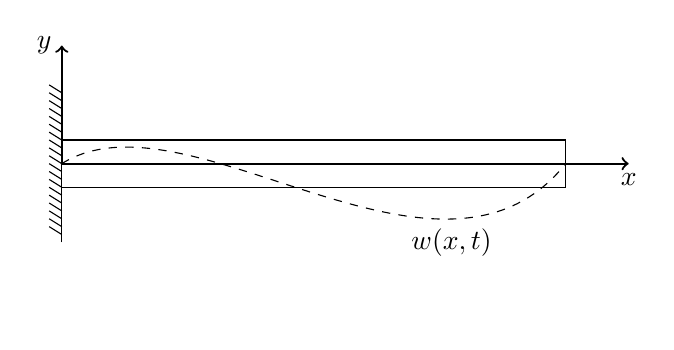
\begin{tikzpicture}[xscale=0.8]

        \draw (0, -0.3) rectangle (8, 0.3);

        \draw[->, thick] (0, 0) -- ++(9, 0) node[below]{$x$};
        \draw[->, thick] (0, 0) -- ++(0, 1.5) node[left]{$y$};
        \draw (0, -1) -- (0,  1);
        \draw[dashed] (0,0) .. controls (2, 1) and (6, -2) .. (8, 0) node[pos=0.75, below]{$w(x,t)$};

        \foreach \y in {-0.9, -0.8, ..., 0.9}
        \draw (0, \y) -- ++(-0.2, +0.1);

    \end{tikzpicture}
    \hspace{1cm}
    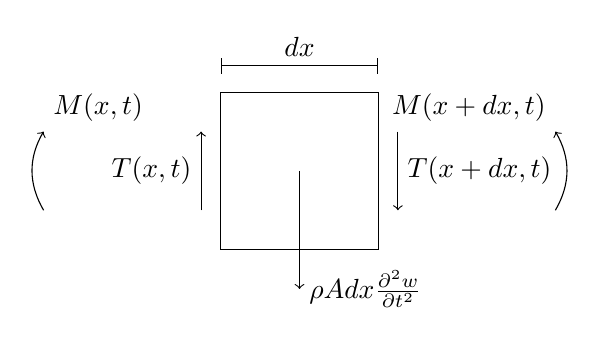
\begin{tikzpicture}

        \def\dx{2}
        \def\dy{2}

        \draw[|-|] (-\dx/2, +4/3*\dy/2) -- ++(\dx, 0) node[midway, above]{$dx$};

        \draw (-\dx/2, -\dy/2) rectangle (\dx/2, \dy/2);
        \draw[->] (0, 0) -- ++(0, -3/4*\dy) node[right]{$\rho A dx\frac{\partial^2 w}{\partial t^2}$};
        \draw[->] (-5/4*\dx/2, -\dy/4) -- ++(0, +1) node[midway, left]{$T(x, t)$};
        \draw[->] (+5/4*\dx/2, +\dy/4) -- ++(0, -1) node[midway, right]{$T(x + dx, t)$};
        \draw[->] (-13/4*\dx/2, -\dy/4) to [bend left] (-13/4*\dx/2, +\dy/4) node[above right]{$M(x, t)$};
        \draw[->] (+13/4*\dx/2, -\dy/4) to [bend right] (+13/4*\dx/2, +\dy/4) node[above left]{$M(x + dx, t)$};

    \end{tikzpicture}

    \caption{Transversal displacement $w(x,t)$ of a beam element and forces acting on infinitesimal element ($dx$).}
    \label{fig:beam_element_forces}

\end{figure}

Using D'Alambert principle, we can write the following vertical and rotational equilibrium for the infinitesimal element represented in Figure \ref{fig:beam_element_forces}:

\begin{equation}
    \begin{matrix}
        -M(x,t) + M(x + dx, t) - T(x,t) \frac{dx}{2} - T(x + dx, t) \frac{dx}{2} = 0 \\
        T(x, t) - T(x + dx, t) = \rho A dx \frac{\partial^2 w}{\partial t^2}
    \end{matrix}
\end{equation}

Using differential calculus, we can rewrite this equilibrium as:

\begin{equation}
    \begin{matrix}
        -M(x,t) + M(x, t) + \frac{\partial M(x,t)}{\partial x} dx - T(x,t) \frac{dx}{2} - T(x,t) \frac{dx}{2} - \frac{\partial T(x,t)}{\partial x} \frac{dx^2}{2} = 0 \\
        T(x, t) - T(x, t) - \frac{\partial T(x, t)}{\partial x} dx = \rho A dx \frac{\partial^2 w}{\partial t^2}
    \end{matrix}
\end{equation}

From which (neglecting higher order terms) we obtain:

\begin{equation}
    \begin{aligned}
        T(x, t)                            & = \frac{\partial M(x,t)}{\partial x}              \\
        \frac{\partial T(x,t)}{\partial x} & = - \rho A \frac{\partial^2 w(x,t)}{\partial t^2}
    \end{aligned}
\end{equation}

Substituting the expression of $T(x,t)$ and recalling the definition of $M(x, t)$ (see Equation \ref{eq:bending_moment_transversal_displacement}), we obtain the following equation of motion for the transversal displacement $w(x,t)$:

\begin{equation}
    \frac{\partial^2}{\partial x^2} \left( EJ \frac{\partial^2 w(x,t)}{\partial x^2} \right) = -\rho A \frac{\partial^2 w(x,t)}{\partial t^2}
    \label{eq:beam_equation_of_motion_transversal_displacement}
\end{equation}

It's easy to recognize that Equation \ref{eq:beam_equation_of_motion_transversal_displacement} is a fourth-order partial differential equation (PDE) in the space variable $x$ and a second-order PDE in the time variable $t$.

In case the material properties are constant both in time and space, $w(x,t)$ can be computed analytically as the product of a spatial function $\alpha(x)$ and a temporal function $\beta(t)$.
However, in the case of non-constant material properties, the problem becomes more complex and numerical methods are usually required to solve it.

\subsection{Piezoelectric patches analysis}
\label{subsec:piezoelectric_patches_analysis}

In this section, we introduce the necessary theory to address the use of piezoelectric patches in the system under investigation.

We start by recalling the general constitutive equations for piezoelectric materials before focusing on the specific case of piezoelectric patches bonded to a beam element.

\begin{figure}[H]
    \centering
    \includegraphics[width=0.5\textwidth]{img/piezo.jpg}
    \caption{Example of piezoelectric patch.}
    \label{fig:piezo}
\end{figure}


\subsubsection{Piezoelectric constitutive equations}
\label{subsubsec:piezoelectric_constitutive_equations}

Piezoelectric materials have the ability to convert mechanical energy into electrical energy and vice versa.
Considering to work within a reasonable range of deformations, the constitutive equations for piezoelectric materials can be linearized and written in matrix form as follows:

\begin{equation}
    \begin{bmatrix}
        \bm{D} \\
        \bm{S}
    \end{bmatrix} =
    \begin{bmatrix}
        \bm{\varepsilon}^T & \bm{d}   \\
        \bm{d}_t           & \bm{s}^E
    \end{bmatrix}
    \begin{bmatrix}
        \bm{E} \\
        \bm{T}
    \end{bmatrix}
\end{equation}

Where $\bm{S} [\Delta m / m]$ and $\bm{D} [C / m^2]$ are the mechanical strain and charge displacement vectors, $\bm{T} [N / m^2]$ and $\bm{E} [N / C]$ are the mechanical stress and electric field vectors, $\bm{s} [1 / Pa]$ is the compliance matrix, $\bm{d} [C / N]$ is the piezoelectric strain coefficient matrix, and $\bm{\varepsilon} [F / m]$ is the dielectric permittivity matrix.
Notice also that the superscript $()^T$ and $()^E$ indicate that the quantities are measured under constant stress and electric field, respectively, while the subscript $t$ indicates the transposition of the matrix.

Taking common assumptions as orthotropy of the material and neglecting any orthogonal piezoelectric effect, the constitutive equations can be greatly simplified forcing many of the coefficients to zero.

For the specific case of piezoelectric patches bonded to a beam element (as will be better shown in Section \ref{subsec:experimental_setup}), we can further simplify the constitutive equations by considering that the electric field is only acting in one direction, and study the stress and strain produced along one of the other normal directions.
In particular, referring to conventional piezoelectric theory, we are interested in the so-called $31$-mode, where the electric field is applied along the $3$-direction and the strain is measured in the $1$-direction (see Figure \ref{fig:piezo_31_operating_mode}).

\begin{figure}[H]
    \centering
    \includegraphics[width=0.7\textwidth]{img/piezo_31_operating_mode.png}
    \caption{Piezoelectric patch operating in $31$-mode.}
    \label{fig:piezo_31_operating_mode}
\end{figure}

Then, under the hypothesis that all the other quantities are zero, the constitutive equations can be written as:

\begin{equation}
    \begin{bmatrix}
        D_3 \\
        S_1
    \end{bmatrix} =
    \begin{bmatrix}
        \varepsilon_{33}^T & d_{31}   \\
        d_{13}             & s_{13}^E
    \end{bmatrix}
    \begin{bmatrix}
        E_3 \\
        T_1
    \end{bmatrix} =
    \begin{bmatrix}
        \varepsilon_{33}^T & d_{31}          \\
        d_{31}             & \frac{1}{Y_1^E}
    \end{bmatrix}
    \begin{bmatrix}
        E_3 \\
        T_1
    \end{bmatrix}
    \label{eq:piezoelectric_constitutive_equations}
\end{equation}

Notice that $\varepsilon_{33}^T$ is the dielectric permittivity in the $3$-direction when the stress in direction $1$ is zero ($T_1 = 0$), and $Y_1^E$ is the Young's modulus in the $1$-direction when the electric field in direction $3$ is zero ($E_3 = 0$).

Equation \ref{eq:piezoelectric_constitutive_equations} can also be rewritten in terms of applied voltage and current by performing the following change of variables and moving to Laplace domain:

\begin{equation}
    \begin{aligned}
        V & = \int_{0}^{L} E \cdot dx & \rightarrow &  & V(s) & = L \cdot E(s)  \\
        I & = \int_A D \cdot dA       & \rightarrow &  & I(s) & = sA \cdot D(s)
    \end{aligned}
\end{equation}

Substituting the expressions for $V$ and $I$ in the constitutive equations, we can obtain the following relationship:

\begin{equation}
    \begin{bmatrix}
        I_3 \\
        S_1
    \end{bmatrix} =
    \begin{bmatrix}
        sC_{3p}^T       & sA_3 d_{31}     \\
        d_{31} L_3^{-1} & \frac{1}{Y_1^E}
    \end{bmatrix}
    \begin{bmatrix}
        V_3 \\
        T_1
    \end{bmatrix}
    \label{eq:piezoelectric_constitutive_equations_volt_current}
\end{equation}

Where $C_p^T = A \varepsilon_{33}^T / L$ is the piezoelectric capacitance per unit length, and $L_3$ is the length of the piezoelectric patch in the $3$-direction.

An important final remark has to be made about the piezoelectric coupling coefficient $k_{31}$, which is defined as:

\begin{equation}
    k_{31} = \frac{d_{31} \sqrt{Y_1^E}}{\varepsilon_{33}^T} = \frac{d_{31}}{\sqrt{\varepsilon_{33}^T Y_1^E}}
\end{equation}

This coefficient is a measure of the efficiency of the piezoelectric material in converting mechanical energy into electrical energy and vice versa.
It's intuitive to understand that $0 < k_{31} < 1$, and the closer it is to $1$, the more efficient the material is in converting energy.


\subsubsection{Shunted piezoelectric patches}
\label{subsubsec:shunted_piezoelectric_patches}

The properties of a piezoelectric patch can be greatly influenced by the presence of a shunt circuit connected to it.
The successive analysis takes as reference the electrical scheme of Figure \ref{fig:shunted_piezoelectric_patch}.

\begin{figure}[H]
    \centering
    \includegraphics[width=0.7\textwidth]{img/piezo_shunted.png}
    \caption{Electrical scheme of a shunted piezoelectric patch.}
    \label{fig:shunted_piezoelectric_patch}
\end{figure}

In order to account for the presence of the shunt circuit, we need to adjust accordingly the electrical impedance of the system, given now as the parallel connection of the piezoelectric patch impedance $Z_p$ and the shunt impedance $Z_{su}$:

\begin{equation}
    Z^{EL} = \left( Z_p^{-1} + Z_{su}^{-1} \right)^{-1}
\end{equation}

% Or equivalently in terms of admittance:

% \begin{equation}
%     Y^{EL} = Z^{EL^{-1}} = Y_p + Y_{su} = sC_p^T + \frac{1}{Z_{su}}
% \end{equation}

Substituting the expression for $Y^{EL}$ in the constitutive equations (Equation \ref{eq:piezoelectric_constitutive_equations_volt_current}), we obtain the following relationship:

\begin{equation}
    \begin{bmatrix}
        I_3 \\
        S_1
    \end{bmatrix} =
    \begin{bmatrix}
        \frac{1}{Z^{EL}} & sA_3 d_{31}     \\
        d_{31} L_3^{-1}  & \frac{1}{Y_1^E}
    \end{bmatrix}
    \begin{bmatrix}
        V_3 \\
        T_1
    \end{bmatrix}
\end{equation}

Solving for the voltage across the piezoelectric patch, and then for the mechanical strain $S$, we can highlight the influence of the shunt circuit on the mechanical properties of the piezoelectric patch.

\begin{equation}
    \begin{aligned}
        V_3 & = Z^{EL} I_3 - Z^{EL} sA_3 d_{31} T_1                                                                                                                             \\
        S_1 & = d_{31} L_3^{-1} V_3 + \frac{1}{Y_1^E} T_1 = \left( d_{31} L_3^{-1} Z^{EL} \right) I_3 + \left( \frac{1}{Y_1^E} - d_{31} L_3^{-1} Z^{EL} sA_3 d_{31} \right) T_1
    \end{aligned}
\end{equation}

Recalling the traditional definition of stress and strain relationship $S = Y^E T$, we can recognize:

\begin{equation}
    \frac{1}{Y^{SU}} = \frac{1}{Y_1^E} - d_{31} L_3^{-1} Z^{EL} sA_3 d_{31}
\end{equation}

Where $Y^{SU}$ is the mechanical admittance of the piezoelectric patch.
It's clear that the presence of the shunt have a direct influence on the mechanical properties of the piezoelectric patch, and thus on the beam element to which it might be bonded.

In the optic of this work, it's of particular interest to obtain a clear equation of the type $Y^{SU} = f(Y_p, Z_{su})$ that can be used to study the influence of the shunt impedance on the mechanical properties of the piezoelectric patch.
In particular, rearranging the terms of the last equation, we can obtain the following expression:

\begin{equation}
    Y^{SU} = Y_1^D \left( 1 - \frac{k_{31}^2}{1 + s C_p^S Z^{SU}} \right)
    \label{eq:mechanical_admittance_shunted_piezoelectric_patch}
\end{equation}


\subsection{Numerical methods for wave propagation analysis}
\label{subsec:numerical_methods_for_wave_propagation_analysis}

In this section, we introduce the numerical methods used to simulate the wave propagation in a generic modulated beam structure.
In particular, one of the main results that can be obtained by using these methods is the dispersion relation of the system, which describes the relationship between the frequency and the wavenumber of the propagating waves.
Once the dispersion relation is known, it is possible to analyze the behavior of the system under different conditions and to design the structure to achieve specific properties as will be shown in the following sections.

The following methods are introduced:

\begin{itemize}
    \item Transfer Matrix Method (TMM): used to analyze the wave propagation in case of purely spatial modulation structure;
    \item Plane Wave Expansion Method (PWEM): allow considering not only space modulation but also time modulation;
    \item Finite Difference Time Domain (FDTD) method: a general-purpose method that can be used to simulate a large family of problems requiring the solution of partial differential equations.
\end{itemize}



\subsubsection{Transfer Matrix Method (TMM)}
\label{subsubsec:transfer_matrix_method_tmm}

One of the most common methods used to analyze the wave propagation in a beam structure is the Transfer Matrix Method (TMM).

The main idea of the TMM is to consider and analyze the system as a series of interconnected elements, each one characterized by a transfer matrix that relates the states at the left and right of the element.
By setting continuity between the states at the boundaries of the elements, and imposing the periodicity of the solution via Floquet theorem, it is possible to obtain the dispersion relation of the system solving an eigenvalue problem.

Given that with the TMM it's not possible to account for time-varying material properties, we limit our analysis to the case of beam structures with spatially varying material properties only, modelled by the following equation of motion:

\begin{equation}
    \frac{\partial^2}{\partial x^2} \left( E J(x) \frac{\partial^2 w(x,t)}{\partial x^2} \right) = - \rho A(x) \frac{\partial^2 w(x,t)}{\partial t^2}
\end{equation}

Based on the equation above, we can define the state vector $y(x)$ as the displacement $w(x,t)$ and its derivatives up to $w^{(3)}(x,t)$.
We can also give a physical interpretation to the state vector considering instead the displacement, slope, bending moment, and shear force of the beam:

\begin{equation}
    y(x) =
    \begin{bmatrix}
        v(x)      \\
        \theta(x) \\
        M(x)      \\
        T(x)
    \end{bmatrix} =
    \begin{bmatrix}
        w(x)                                     \\
        \frac{\partial w(x)}{\partial x}         \\
        -EJ \frac{\partial^2 w(x)}{\partial x^2} \\
        -EJ \frac{\partial^3 w(x)}{\partial x^3}
    \end{bmatrix}
\end{equation}

Once the state vector is defined, we write the governing equation of motion in the state-space form:

\begin{equation}
    \frac{\partial y(x)}{\partial x} = A(x) y(x) =
    \begin{bmatrix}
        0                  & 1 & 0                & 0 \\
        0                  & 0 & \frac{-1}{EJ(x)} & 0 \\
        0                  & 0 & 0                & 1 \\
        \omega^2 \rho A(x) & 0 & 0                & 0
    \end{bmatrix} y(x)
\end{equation}

Where $\omega$ is the angular frequency of the travelling wave in the beam.
The solution of the equation above can be written as:

\begin{equation}
    y(x) = T(x) y(0) = e^{x A(x)} y(0)
\end{equation}

Imposing now the continuity of the states at the boundaries of the elements, we can write the transfer matrix of the system as:

\begin{equation}
    T = T(x_r) T(x_{r-1}) \ldots T(x_1) = \prod_{i=r}^{1} T(x_i)
\end{equation}

Which leads to the following periodicity condition in space:

\begin{equation}
    y(x + \lambda_m) = T y(x)
\end{equation}

Notice, however, that the Floquet theorem can also be used to impose periodicity in space, and combined with the above equation, it leads to the following eigenvalue problem:

\begin{equation}
    \begin{aligned}
        y(x + \lambda_m) & = T y(x)         \\
        y(x + \lambda_m) & = e^{i \mu} y(x)
    \end{aligned}
    \rightarrow
    T y(x) = e^{i \mu} y(x)
    \label{eq:transfer_matrix_method_eigenvalue_problem}
\end{equation}

Where $\mu$ is the Floquet exponent or the non-dimensional wavenumber, and it can be used to obtain the dispersion relation of the system given that $\mu = \kappa \lambda_m$.

It's clear how the TMM corresponds to an inverse solution for the dispersion, given that the eigenvalue problem in Equation \ref{eq:transfer_matrix_method_eigenvalue_problem} can be solved to obtain the Floquet exponent $\mu$ as a function of the angular frequency $\omega$, on which $T$ depends.



\subsubsection{Plane Wave Expansion Method (PWEM)}
\label{subsubsec:plane_wave_expansion_method_pwem}

The Plane Wave Expansion Method (PWEM) is a numerical method used to solve plane waves in periodic structures.
Its more general version, often referred to as Generalized Plane Wave Expansion Method (GPWEM), allows for the analysis of waves without any restriction on the form of the wave itself.
The main advantage with respect to the TMM is that the PWEM can be used to analyze not only spatially varying material properties but also time-varying ones.

The idea here is to move to the frequency domain via Fourier series expansion and, upon the imposition of the periodicity of the solution via Floquet theorem, to solve the wave equation which will now be in the form of a Quadratic Eigenvalues Problem (QEP).
A main difference with respect to the TMM is that the solution of the PWEM is a direct one, meaning that the dispersion relation is obtained by imposing the wavenumber $\kappa$ and solving for the frequency $\omega$.

For the problem at hand, we consider dealing with structural beam properties varying both in space and in time, with a periodicity dictated by $\lambda_m$ and $T_m$ respectively.
The Fourier series expansion of the structural properties then reads:

\begin{equation}
    \begin{aligned}
        \begin{aligned}
            EJ(x, t) & = \sum_{m,n} \left[ \frac{1}{\lambda_m T_m} \int_{-\frac{\lambda_m}{2}}^{\frac{\lambda_m}{2}} \int_{-\frac{T_m}{2}}^{\frac{T_m}{2}} EJ(x, t) e^{-i (m\kappa_m x - n\omega_m t)}dx dt \right] e^{i (m\kappa_m x - n\omega_m t)} \\
                     & = \sum_{m,n} \widehat{EJ}_{m,n} e^{i (m\kappa_m x - n\omega_m t)}
        \end{aligned} \\
        \begin{aligned}
            \rho A(x, t) & = \sum_{m,n} \left[ \frac{1}{\lambda_m T_m} \int_{-\frac{\lambda_m}{2}}^{\frac{\lambda_m}{2}} \int_{-\frac{T_m}{2}}^{\frac{T_m}{2}} \rho A(x, t) e^{-i (m\kappa_m x - n\omega_m t)}dx dt \right] e^{i (m\kappa_m x - n\omega_m t)} \\
                         & = \sum_{m,n} \widehat{\rho A}_{m,n} e^{i (m\kappa_m x - n\omega_m t)}
        \end{aligned}
    \end{aligned}
\end{equation}

With similar fashion, we can impose the Floquet solution to the displacement $w(x, t)$ and expand it in the frequency domain as:

\begin{equation}
    w(x, t) = e^{i (\kappa x - \omega t)} \sum_{p, q} \widehat{w}_{p,q} e^{i (p\kappa_m x - q\omega_m t)}
\end{equation}

After some nontrivial algebraic manipulations, that include the integration over the space and time domains and the application of the orthogonality of the Fourier series, the wave equation can be rewritten in the following form:

\begin{equation}
    \sum_{p, q} \left( p \kappa_m + \kappa \right)^2 \left( s \kappa_m + \kappa \right)^2 \widehat{EJ}_{s-p, r-q} \widehat{w}_{p,q} = \sum_{p, q} \left( q \omega_m + \omega \right) \left( r \omega_m + \omega \right) \widehat{\rho A}_{s-p, r-q} \widehat{w}_{p,q}
    \label{eq:plane_wave_expansion_method_wave_equation}
\end{equation}

Equation \ref{eq:plane_wave_expansion_method_wave_equation} is basically the equivalent of Equation \ref{eq:beam_equation_of_motion_transversal_displacement} in the frequency domain, considering $P$ and $Q$ as the number of harmonics in space and time respectively.

The solution of Equation \ref{eq:plane_wave_expansion_method_wave_equation} can be obtained by solving the Quadratic Eigenvalues Problem (QEP) associated to Equation \ref{eq:plane_wave_expansion_method_wave_equation} for the frequency $\omega$ as a function of the wavenumber $\kappa$.
In particular, the QEP can be written as:

\begin{equation}
    \left( \omega^2 L_2 (\kappa) + \omega L_1 (\kappa) + L_0 (\kappa) \right) \widehat{w} = 0
\end{equation}

Where $L_2 (\kappa)$ and $L_1 (\kappa)$ are in some sense associated to the mass matrices of the system, while $L_0 (\kappa)$ represent the equivalent stiffness matrix given as a summation of contributions relative to both the flexural stiffness ($EJ$) and the inertial properties ($\rho A$) of the beam.
Notice also that the size of the QEP is $(2Q + 1)\times(2P + 1)$, which can be bottleneck in terms of computational resources given that it should be solved for each value of the wavenumber $\kappa$.



\subsubsection{Finite Difference Time Domain (FDTD) method}
\label{subsubsec:finite_difference_time_domain_fdtd_method}

The Finite Difference Time Domain (FDTD) method is a general-purpose method used to solve partial differential equations.
It operates by discretizing both the spatial and temporal domains and approximating differential operators using finite differences.

By adopting a Taylor series expansion, the second-order and fourth-order finite difference approximations for a function $f(x)$ are given by:

\begin{equation}
    \frac{\partial^2 f(x)}{\partial x^2} \approx \frac{f(x + \Delta x) - 2 f(x) + f(x - \Delta x)}{\Delta x^2}
    \label{eq:finite_difference_second_order}
\end{equation}

\begin{equation}
    \frac{\partial^4 f(x)}{\partial x^4} \approx \frac{f(x + 2 \Delta x) - 4 f(x + \Delta x) + 6 f(x) - 4 f(x - \Delta x) + f(x - 2 \Delta x)}{\Delta x^4}
    \label{eq:finite_difference_fourth_order}
\end{equation}

As done in the Section \ref{subsubsec:plane_wave_expansion_method_pwem}, we can consider a beam structure with properties varying both in space and in time (periodicity dictated by $\lambda_m$ and $T_m$ respectively).

One could directly apply the finite difference method to Equation \ref{eq:beam_equation_of_motion_transversal_displacement}, but this would require to compute the displacement in a given cell based on the derivative of the displacement of the neighboring cells.
Instead, in order to avoid relying on possibly cumulative approximations, we introduce a dummy variable $v(x,t)$ such that its second spatial derivative corresponds to the displacement $w(x,t)$.
The problem can now be rewritten as:

\begin{equation}
    \begin{cases}
        EJ(x, t) \frac{\partial^4 v(x,t)}{\partial x^4} = - \rho A(x, t) \frac{\partial^2 v(x,t)}{\partial t^2} \\
        w(x,t) = \frac{\partial^2 v(x,t)}{\partial x^2}
    \end{cases}
\end{equation}

Discretizing the space and time domains and applying finite difference approximations (Equations \ref{eq:finite_difference_second_order} in time and \ref{eq:finite_difference_fourth_order} in space), we derive the following set of update equations:

\begin{equation}
    \begin{cases}
        \begin{aligned}
            v(t + \Delta t, x) = &
            -\left( \frac{c(x, t)^2 \Delta t}{\Delta x^2} \right)^2
            \left[ v(t, x + 2\Delta x) - 4 v(t, x + \Delta x) + 6 v(t, x) - 4 v(t, x - \Delta x) + v(t, x - 2\Delta x) \right] + \\
                                 & + 2 v(t, x) - v(t - \Delta t, x)                                                              \\
        \end{aligned} \\
        w(t + \Delta t, x) = \frac{1}{\Delta x^2} \left[ v(t + \Delta t, x + \Delta x) - 2 v(t + \Delta t, x) + v(t + \Delta t, x - \Delta x) \right]
    \end{cases}
\end{equation}

Where $c(x, t) = (EJ(x, t) / \rho A(x, t))^{1/4}$ is the equivalent traversal wave speed in the beam.


\paragraph{Boundary conditions}

Boundary conditions can be enforced by setting appropriate values for the displacement and dummy variable at the domain limits.
Dirichlet boundary conditions, for instance, can be implemented by setting the displacement to zero at the boundaries ($w(t, x_{min}) = w(t, x_{max}) = 0$).

On the other hand, given that we are dealing with finite domains, it's also important to avoid or at least minimize the reflection of the waves at the boundaries.
To do so, one can simply introduce a buffer zone along the space dimension with properties equal to the ones of the beam structure so that the waves can travel through it without being reflected back in the domain of interest.
Simulation time can also be tuned in order to minimize the reflection of the waves back from the boundaries.

Excitation forces can be imposed at selected points by modifying the values of the displacement and the dummy variable at the corresponding locations at each time step of the simulation.


\paragraph{Stability condition}

The numerical stability of the FDTD method is governed by the Courant-Friedrichs-Lewy (CFL) condition, which dictates the maximum allowable time step to ensure stable wave propagation.
The idea is that the simulated wave should not travel faster than the speed of the wave in the real system.

The CFL condition is given by:

\begin{equation}
    \left( \frac{max|c(x, t)^2| \Delta t}{\Delta x^2} \right)^2 \leq C_{max}
\end{equation}

Where $C_{max}$ is a constant that depends on the specific problem under investigation, but it that can be set to $1$ in most cases.

